
\section{Code Structure}

\setcounter{equation}{0}

A flow diagram of the PFLOTRAN code structure is shown in Figure~\ref{fdiag}.

\begin{figure}[h]\centering
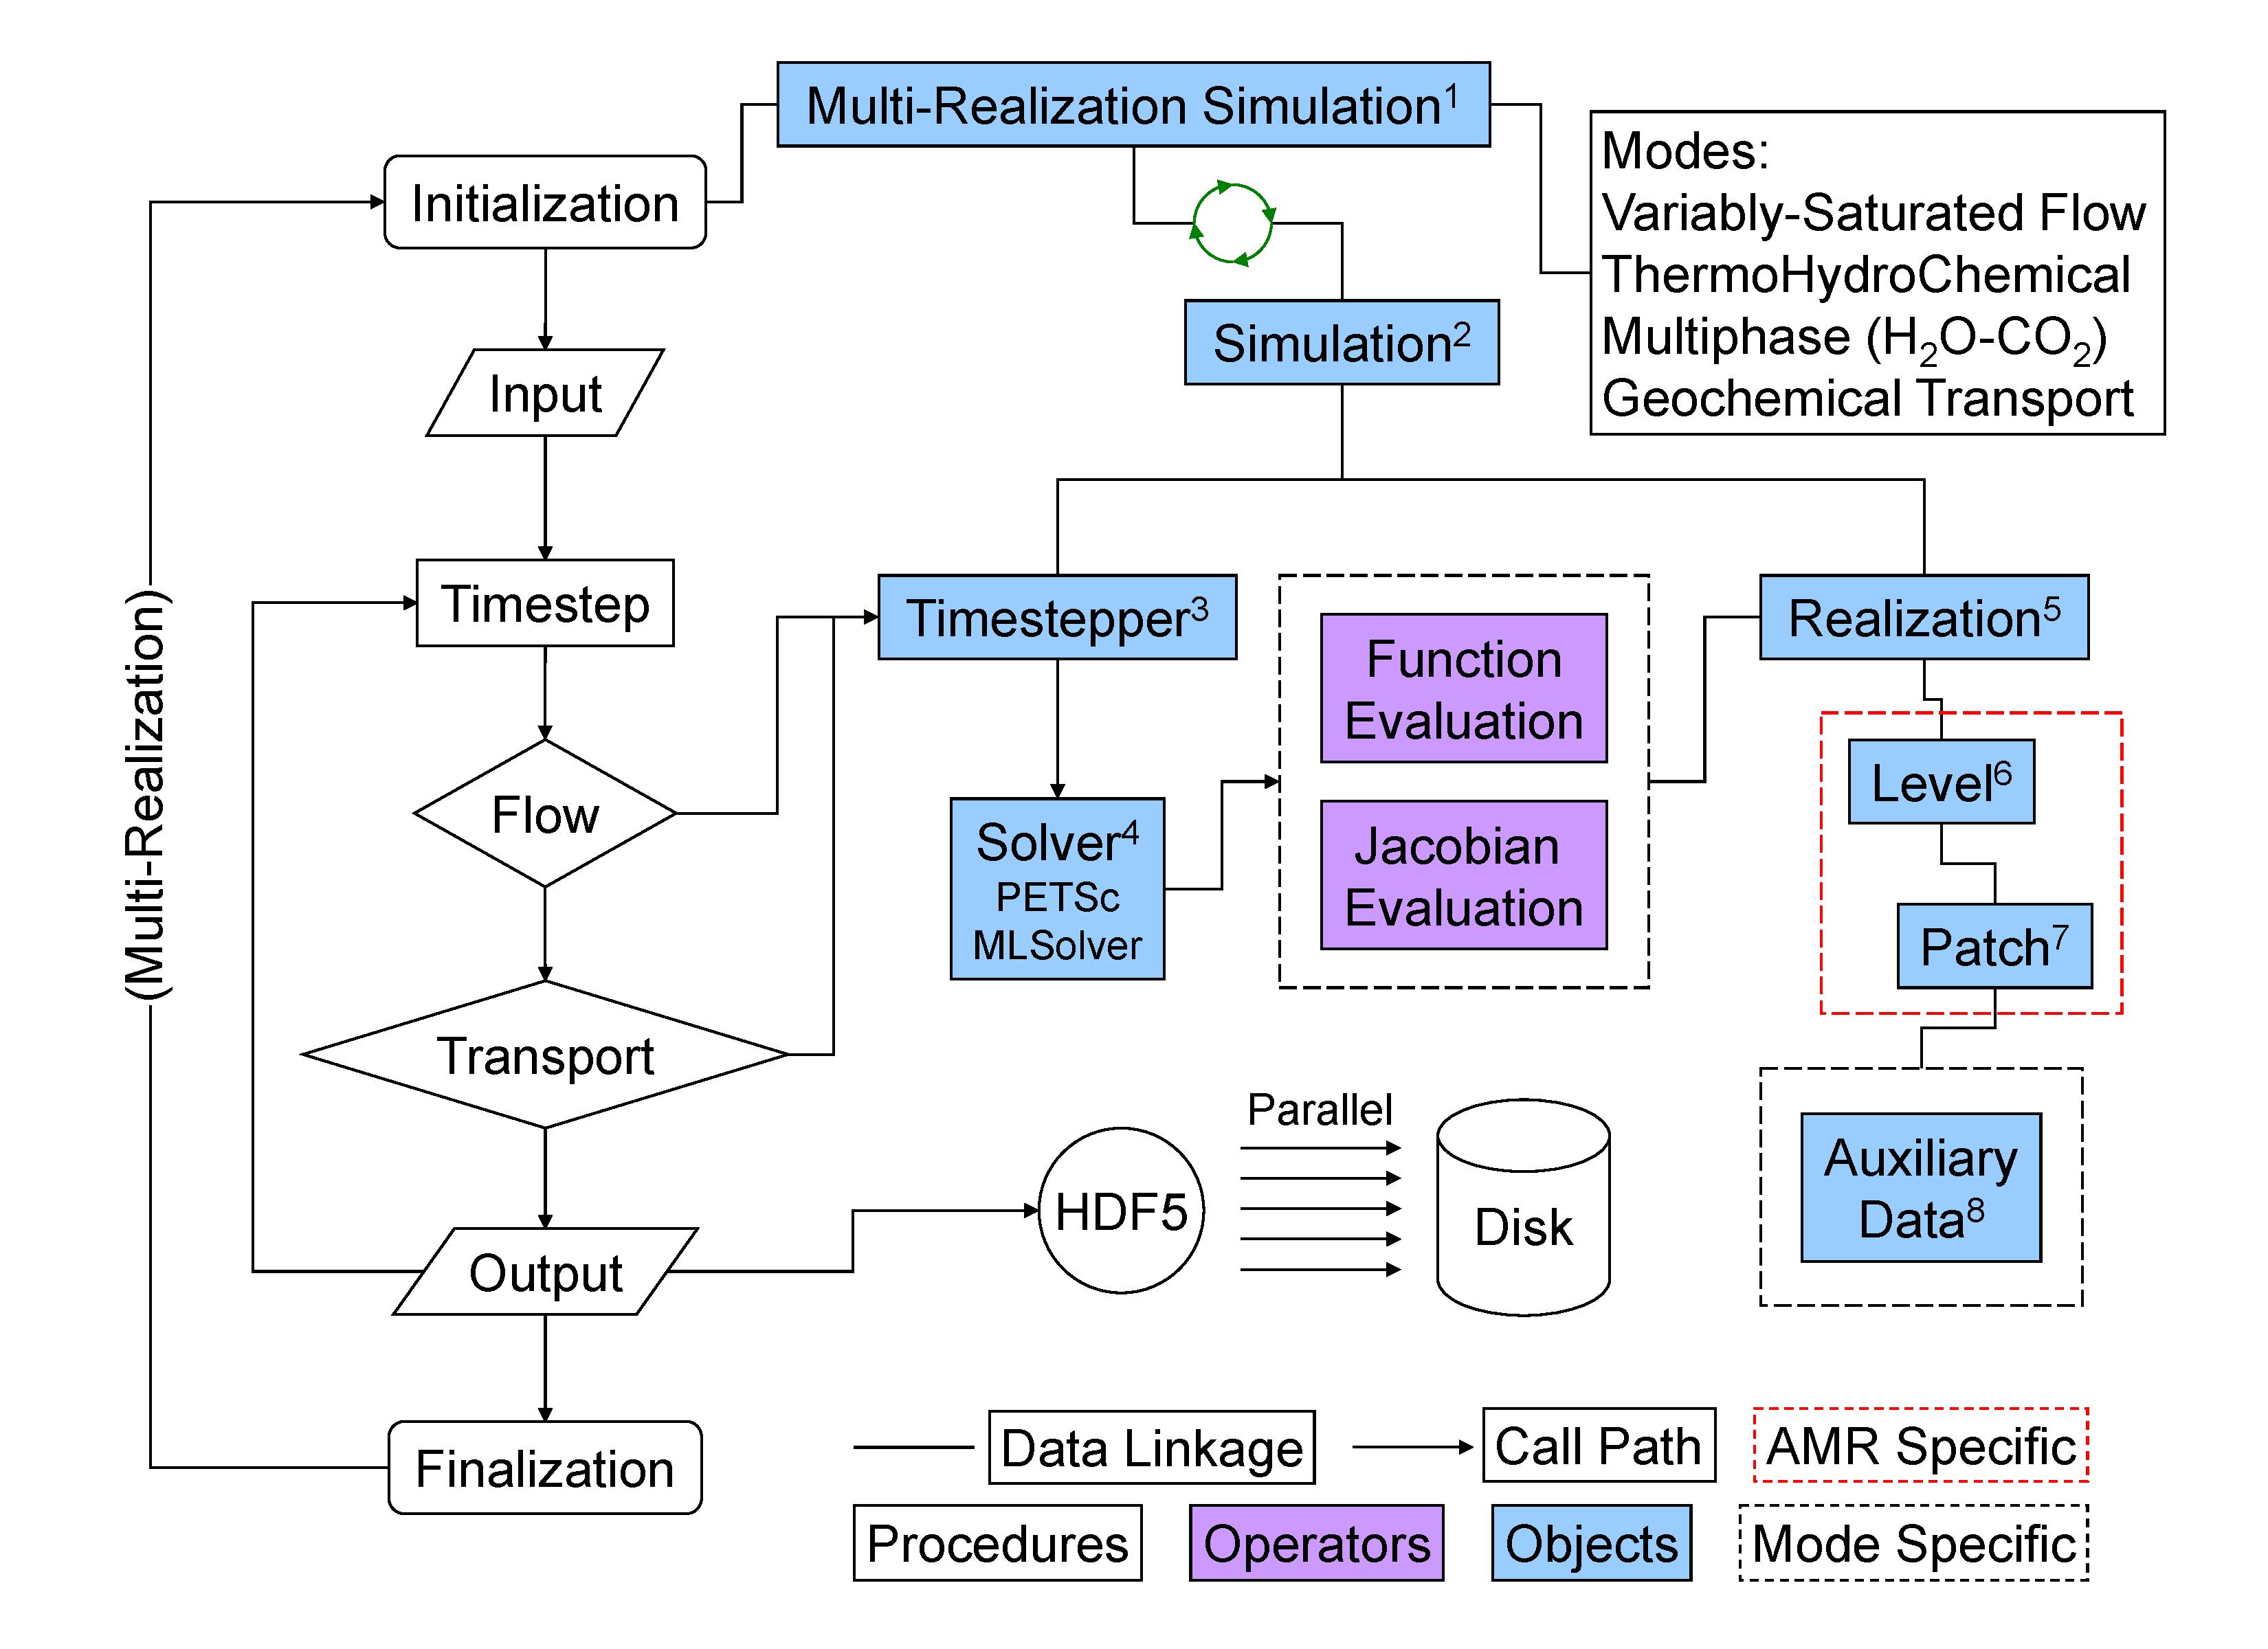
\includegraphics[scale=0.3]{./figs/multi-realization_flowchart}
\caption{Flow diagram of PFLOTRAN illustrating use of procedures, operators, and objects.}\label{fdiag}
\end{figure}

Flow diagram definitions:
\begin{enumerate}
\item {\bf Multi-Realization Simulation} object: Highest level data structure providing all information for running simulations composed of multiple realizations
\item {\bf Simulation} object: Data structure providing all information for running a single simulation
\item {\bf Timestepper} object: Pointer to Newton-Krylov solver and tolerances associated with time stepping
\item {\bf Solver} object: Pointer to nonlinear Newton and linear Krylov solvers (PETSc) along with associated convergence criteria
\item {\bf Realization} object: Pointer to all discretization and field variables associated with a single realization of a simulation
\item {\bf Level} object: Pointer to discretization and field variables associated with a single level of grid refinement within a realization
\item {\bf Patch} object: Pointer to discretization and field variables associated with a subset of grid cells within a level
\item {\bf Auxiliary Data} object: Pointer to auxiliary data within a realization/patch
\end{enumerate}


In order to facilitate code development and better preserve the extensibility and modularity of the code, an object-oriented coding paradigm is employed within PFLOTRAN.  In comparison to traditional procedural paradigms, the object-oriented programming paradigm facilitates code modification and reuse.  Within the context of PFLOTRAN, the utilization of this paradigm greatly accelerates the incorporation of new flow and transport modes through the extension of existing algorithms.  The compartmentalization of methods, processes and data enables the spawning of multi-realization simulations, each of which can be simultaneously run in parallel (i.e. each realization of the multi-realization simulation can be run in parallel utilizing multiple processor cores).

